\documentclass{article}
\usepackage[utf8]{inputenc}
\usepackage[spanish]{babel}
\usepackage{listings}
\usepackage{graphicx}
\graphicspath{ {images/} }
\usepackage{cite}

\begin{document}

\begin{titlepage}
    \begin{center}
        \vspace*{1cm}
            
        \Huge
        \textbf{Taller- Nociones de la memoria del computador}
            
        \vspace{0.5cm}
        \LARGE
        
            
        \vspace{1.5cm}
            
        \textbf{Ana Cristina Henao Guerra}
        
        \textbf{cc. 103767030}
            
        \vfill
            
        \vspace{0.8cm}
            
        \Large
        Despartamento de Ingeniería Electrónica y Telecomunicaciones\\
        Universidad de Antioquia\\
        Medellín\\
        Septiembre de 2020
            
    \end{center}
\end{titlepage}

\tableofcontents
\newpage
\section{Sección introductoria}\label{intro}
Esta es la primera sección, podemos agregar algunos elementos adicionales y todo será escrito correctamente. Más aún, si una palabra es demasiado larga y tiene que ser truncada, babel tratará de truncarla correctamente dependiendo del idioma.

\section{Sección de contenido} \label{contenido}
Dando solución a las siguientes preguntas definidas previamente en el taller, con base en la lectura propuesta por el profesor Augusto Salazar.\\
%
1. Defina que es la memoria del computador.\\
2.Mencione 2 tipos de memoria que conoce y haga una pequeña descripción de cada tipo.\\
3. Describa la manera como se gestiona la memoria en un computador.\\
4. ¿Que hace que una memoria sea más rápida que otra? ¿Por qué esto es importante?


\subsection{Defina que es la memoria del computador}
%
La memoria del computador, es un dispositivo donde se almacena temporalmete toda la información con la que posteriormente hacen uso los demás dispositivos del computador, como son los microprocesadores y éstos se encargan de procesarla y usarla, de tal manera que se obtenan los resultados que el usuario esta esperando.


\subsection{Mencione 2 tipos de memoria que conoce y haga una pequeña descripción de cada tipo}
%
Memoria RAM: por sus siglas en inglés Random Access Memory (acceso de memoria aleatoria). Esta memoria se encuentra dividida en celdas (de ahí su nombre), en cada una, se almacena temporalmente la información; más específicamente bits (1 o 0) ó pulsos eléctricos a los cuales se tiene acceso direto sin importar su dirección o posición.
Cada celda que compone la memoria RAM está compuesta por un transistor y capacitor de tamaño microscópico.
la funcion de los capacitores, es sotener los bits de información y la de los transistores, es permitir al controlador de memoria leer o incluso modificar la información almacenada en cada una de las celdas.

los capacitores deben ser cargados constantemente con electrones que representan la información, ya que tienden a 'vaciarse' en cuestión de pocos milisegundos. Para que éste proceso de 'carga' se lleve a cabo, el controlador primero debe leer la memoria y procede a llenar los capacitores que aun están cargados para evitar el "vaciado" anteriormente mencionado.\\
%
\begin{figure}[h]
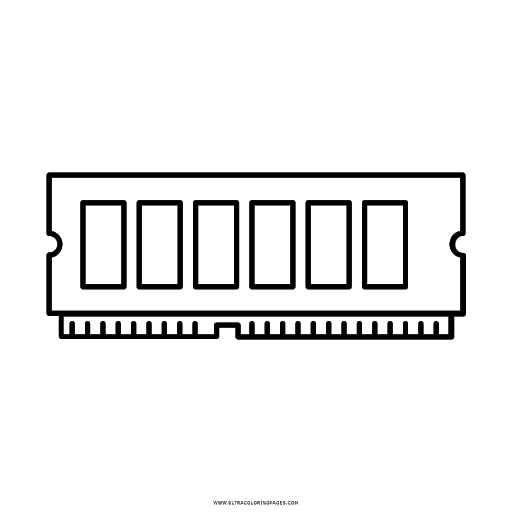
\includegraphics[width=4cm]{memoriaRAM.png}
\centering
\caption{imagen memoria RAM}
\label{fig:memoriaRAM}
\end{figure}

Memoria virtual: Es una parte del disco duro que es previamente reservada para almacenar temporalmente informacíon que ocupa espacio innecesario de la memoria como fragmentos de programas que son menos utilizados. La información allí almacenada está siempre disponible para cuando requiera ser utilizada. 

la memoria virtual, nace como solución al uso excesivo de memoria RAM, cuando se usan simultaneamente programas que ocupan mucho espacio en su ejecución al pasar la información a un 'segundo plano' mientras no se esté usando.
A pesar de ser éste un buen recurso, la solución para tener un mejor rendimiento en el equipo, es tener la mayor cantidad de memoria RAM posible y disponible.
 
\subsection{¿Como se gestiona la memoria de un computador?}
%
La forma de gestión de memoria, refiere al almacenamiento temporal de información con la que trabajan los microprocesadores, en donde la procesan y devuelven los resultados pedidos por el usuario.

En principio, el disco duro se encarga de llevar la información hasta una parte de la memoria, para que el microprocesador proceda a realizar las tareas necesarias, y luegola información pase a otro lugar de la memoria, donde se almacenará esa información procesada.
Cuando este ciclo se repita todas las veces necesarias, toda la información previamente procesada, vuelve a ser guardada en el disco duro.

\subsection{¿Que hace que una memoria sea más rápida que otra?}
%
La información y las instrucciones que se encuentran almacenadas en las memorias del computador, viajan a través de un bus de datos, que son circuitos en cobre que reposan sobre la tarjeta o también llamada "placa madre", que es una tarjeta en la cual se conecta los circutos que conforman el computador.
La velocidad con la que se permite el acceso a la información guardada en cada memoria, depende también de la cantidad de bits o de pulsos eléctricos que se transfieran a través del bus, o sea entre una memoria u otra.
En síntesis, lo que hace que una memoria sea más rápida, es la cantidad de información que se almacena en cada una, dependiendo también de su tipo. 


\section{Inclusión de imágenes} \label{imagenes}

En la Figura (\ref{fig:memoriaRAM}), se presenta la imagen de una memoria RAM

\bibliographystyle{IEEEtran}
\bibliography{references}

\end{document}
